% TikZ-reproduction of fig. 1 from the paper MADE: Masked Autoencoder for Distribution Estimation (https://arxiv.org/abs/1502.03509).

\documentclass[tikz]{standalone}

\usepackage{xstring}

\usetikzlibrary{calc,positioning}

\newcommand\drawNodes[2]{
  % #1 (str): namespace
  % #2 (list[list[str]]): list of labels to print in the node of each neuron
  \foreach \neurons [count=\lyrIdx] in #2 {
    \StrCount{\neurons}{,}[\lyrLength] % use xstring package to save each layer size into \lyrLength macro
    \foreach \n [count=\nIdx] in \neurons
      \node[neuron] (#1-\lyrIdx-\nIdx) at (\lyrLength/2-\nIdx, 1.5*\lyrIdx) {\n};
  }
}

\newcommand\denselyConnectNodes[2]{
  % #1 (str): namespace
  % #2 (list[int]): number of nodes in each layer
  \foreach \n [count=\lyrIdx, remember=\lyrIdx as \previdx, remember=\n as \prevn] in #2 {
    \foreach \y in {1,...,\n} {
      \ifnum \lyrIdx > 1
        \foreach \x in {1,...,\prevn}
          \draw[->] (#1-\previdx-\x) -- (#1-\lyrIdx-\y);
      \fi
    }
  }
}

\newcommand\connectSomeNodes[2]{
  % #1 (str): namespace
  % #2 (list[list[list[int]]]): for each node in each layer, list all connected nodes in the next layer
  \foreach \layer [count=\lyrIdx, evaluate=\lyrIdx as \nextLyr using int(\lyrIdx+1)] in #2
    \foreach \neuron [count=\nIdx] in \layer
        \foreach \edge in \neuron
          \draw[->] (#1-\lyrIdx-\nIdx) -- (#1-\nextLyr-\edge);
}

\begin{document}
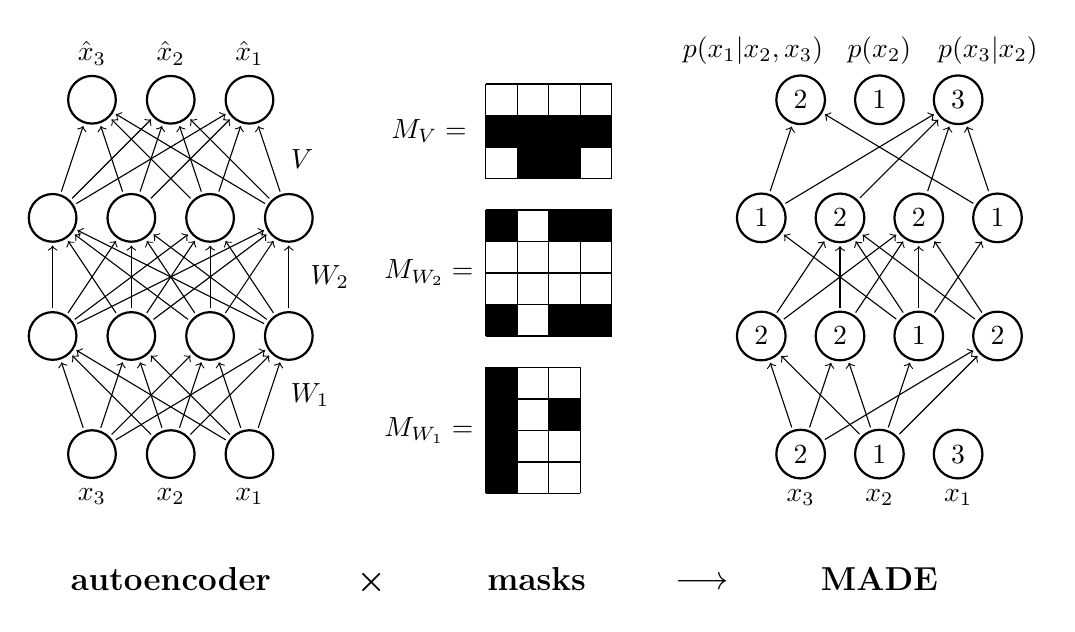
\begin{tikzpicture}[
    shorten >=1pt, shorten <=1pt,
    neuron/.style={circle, draw, minimum size=4ex, thick},
    legend/.style={font=\large\bfseries},
  ]

  % Fully-connected neural net
  \drawNodes{fcnn}{{{,,}, {,,,}, {,,,}, {,,}}}
  \denselyConnectNodes{fcnn}{{3, 4, 4, 3}}

  \path (fcnn-1-1) -- (fcnn-2-1) node[midway, right=1ex] (W1) {$W_1$};
  \path (fcnn-2-1) -- (fcnn-3-1) node[midway, right=1ex] (W2) {$W_2$};
  \path (fcnn-3-1) -- (fcnn-4-1) node[midway, right=1ex] (V) {$V$};


  % MADE net
  \begin{scope}[xshift=9cm]
    \drawNodes{made}{{{3,1,2}, {2,1,2,2}, {1,2,2,1}, {3,1,2}}}
    \connectSomeNodes{made}{{
          {{}, {1,2,3,4}, {1,3,4}},
          {{2,3}, {1,2,3,4}, {2,3}, {2,3}},
          {{1,3}, {1}, {1}, {1,3}},
        }}
  \end{scope}

  % Input + output labels
  \foreach \idx in {1,2,3} {
      \node[below=0 of fcnn-1-\idx] {$x_\idx$};
      \node[above=0 of fcnn-4-\idx] {$\hat x_\idx$};
      \node[below=0 of made-1-\idx] {$x_\idx$};
    }

  % MADE output labels
  \node[xshift=2.5ex, above=0 of made-4-1] {$p(x_3|x_2)$};
  \node[above=0 of made-4-2] {$p(x_2)$};
  \node[xshift=-4ex, above=0 of made-4-3] {$p(x_1|x_2,x_3)$};

  % Bottom legend
  \node[legend, below=of fcnn-1-2] (encoder) {autoencoder};
  \node[legend, below=of made-1-2] (made) {MADE};
  \node[legend, right=2.5cm of encoder] (masks) {masks};
  \node[legend, yshift=-1pt] (masks) at ($(encoder)!0.55!(masks)$) {\texttimes};
  \node[legend, yshift=-1pt] (masks) at ($(masks)!0.65!(made)$) {$\longrightarrow$};

  % Mask matrices
  \begin{scope}[shift={(3cm,5cm)}, scale=0.4]
    \draw (0,0) grid (4,3);
    \node at (-1.8,1.5) {$M_V =$};
    \fill[black] (0,1) rectangle ++(4,1);
    \fill[black] (1,0) rectangle ++(2,1);

    \begin{scope}[yshift=-5cm]
      \draw (0,0) grid (4,4);
      \node at (-1.8,2) {$M_{W_2} =$};
      \fill[black] (0,0) rectangle ++(1,1);
      \fill[black] (0,3) rectangle ++(1,1);
      \fill[black] (2,0) rectangle ++(2,1);
      \fill[black] (2,3) rectangle ++(2,1);
    \end{scope}

    \begin{scope}[yshift=-10cm]
      \draw (0,0) grid (3,4);
      \node at (-1.8,2) {$M_{W_1} =$};
      \fill[black] (0,0) rectangle ++(1,4);
      \fill[black] (2,2) rectangle ++(1,1);
    \end{scope}

  \end{scope}

\end{tikzpicture}
\end{document}
